%:
\documentclass[11pt, oneside]{article}   	% use "amsart" instead of "article" for AMSLaTeX format
\usepackage{geometry}                		% See geometry.pdf to learn the layout options. There are lots.
\geometry{letterpaper}                   		% ... or a4paper or a5paper or ... 
%\geometry{landscape}                		% Activate for rotated page geometry
%\usepackage[parfill]{parskip}    		% Activate to begin paragraphs with an empty line rather than an indent
\usepackage{graphicx}				% Use pdf, png, jpg, or eps§ with pdflatex; use eps in DVI mode
								% TeX will automatically convert eps --> pdf in pdflatex		
\usepackage{amssymb}
\usepackage{diagbox}
\usepackage{amsmath}
\usepackage{amsthm}
\usepackage{enumerate}
\usepackage{tikz}
\usetikzlibrary{positioning}


\usetikzlibrary{arrows}
\theoremstyle{definition}
\newtheorem*{defn}{Definition}
\newtheorem*{prop}{Proposition}
\newtheorem*{eg}{Example}
\newtheorem*{thm}{Theorem}
\newtheorem*{corol}{Corollary}
\newtheorem{ex}{Exercise}[section]
{\theoremstyle{plain}
\newtheorem*{rmk}{Remark}
\newtheorem*{rmks}{Remarks}
\newtheorem*{lt}{Last time}
}
\newtheorem*{lem}{Lemma}
\usepackage{color}
\usepackage{CJK}
\title{Path to Efficient AGI}
\author{Xiyu Zhai}
\date{}							% Activate to display a given date or no date

\begin{document}
\maketitle
\tableofcontents

\section{Introduction}

This paper is the prelude of a series of papers that explore a new school of AI methodologies of a different nature than any existing ones. By combining these new ideas with established AI methods like deep learning, we will be making significant progress towards \textbf{efficient} artificial general intelligence.

Here \textbf{efficient} is stressed upon because we believe this is the key, which is largely missing in other discussions of AGI (I might be wrong, because I didn't read them). Specifically, the meaning of \textbf{efficiency} is twofold:

\begin{enumerate}[(i)]
	\item Statistical efficiency. The ability to learn accurately from limited examples. This is an area what biological intelligence excels yet deep learning struggles.
	\item Computational efficiency. The ability to perform computation in time and within resource boundary. Biological intelligence are good at it if the computation is critical for survival, whereas deep learning has to use large amount of computation resources to match with human in many tasks.
\end{enumerate}

\begin{rmk}
	Biological intelligence, with human intelligence being the most prominant, is still far from perfection. We are already beaten by computers in terms of memory, rule based computation.
\end{rmk}

\section{Related Works}



\section{Theories}

\subsection{Conventions}

For the matter of succinctness, we shall restrict ourselves to Turing machine level when thinking of computation. This is of course far from reality, but it helps with illuminating the high level ideas.


\subsection{NP Problems Arising from ML Problems}

\subsection{ML Problems Arising from NP Problems}
\begin{center}
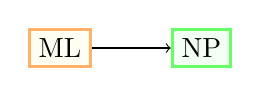
\begin{tikzpicture}[
roundnode/.style={rectangle, draw=green!60, fill=green!5, very thick, minimum size=4mm},
squarednode/.style={rectangle, draw=orange!60, fill=yellow!5, very thick, minimum size=4mm},
]
%Nodes
\node[squarednode]      (ml0)                              {$\text{ML}$};
\node[roundnode]        (np1)       		[right=of ml0] {$\text{NP}$};

%Lines
\draw[->] (ml0.east) -- (np1.west);
\end{tikzpicture}
\end{center}

\subsection{NP-ML Ascension}
\begin{center}
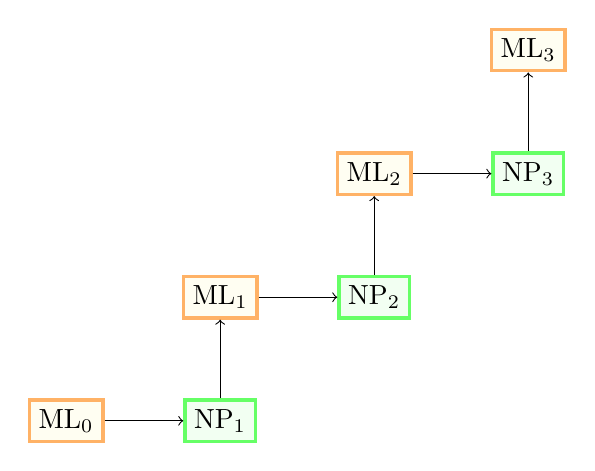
\begin{tikzpicture}[
roundnode/.style={rectangle, draw=green!60, fill=green!5, very thick, minimum size=4mm},
squarednode/.style={rectangle, draw=orange!60, fill=yellow!5, very thick, minimum size=4mm},
]
%Nodes
\node[squarednode]      (ml0)                              {$\text{ML}_0$};
\node[roundnode]        (np1)       		[right=of ml0] {$\text{NP}_1$};
\node[squarednode]      (ml1)       		[above=of np1] {$\text{ML}_1$};
\node[roundnode]        (np2)       		[right=of ml1] {$\text{NP}_2$};
\node[squarednode]      (ml2)       		[above=of np2] {$\text{ML}_2$};
\node[roundnode]        (np3)       		[right=of ml2] {$\text{NP}_3$};
\node[squarednode]      (ml3)       		[above=of np3] {$\text{ML}_3$};

%Lines
\draw[->] (ml0.east) -- (np1.west);
\draw[->] (np1.north) -- (ml1.south);
\draw[->] (ml1.east) -- (np2.west);
\draw[->] (np2.north) -- (ml2.south);
\draw[->] (ml2.east) -- (np3.west);
\draw[->] (np3.north) -- (ml3.south);
\end{tikzpicture}
\end{center}

\subsection{Reinforcement Learning}


\section{Type System}

\subsection{Concept Level Types}


\subsection{System Level Types}

\subsection{Types for Machine Learning}

\section{Language Requirements}

\section{System}

\subsection{Database}

\subsection{Debugger}

\subsection{todo}

\end{document}